% ---------------------------------------------------------------------
%  Chapter 2 : A Worked Example, End to End
% ---------------------------------------------------------------------
\chapter{A Worked Example, End to End}\label{ch:quickstart}

This chapter is your first hands-on contact with the engine. We will take a
single, small, genuinely nonlinear stochastic model --- a quartic
Ornstein--Uhlenbeck particle driven by white noise --- and carry it the whole
way from a one-line model name to a plotted correlation function with an
independent simulator drawn on top. Nothing is hidden: every line of code is
shown, every printed line of output is quoted, and the few numbers that matter
(the equal-time variance the theory predicts, and the one the simulation
measures) are compared side by side.

The point of starting here, before any of the machinery chapters, is to give
you a mental ``spine'' for the rest of the manual. By the end of this chapter
you will have seen the four verbs that drive everything --- \code{load\_theory},
\code{Config}, \code{run}, \code{plot\_cumulant} --- and you will have watched
the engine narrate its own seven internal phases. Later chapters open up each of
those phases in turn; this one just runs them.

The model we use is the one shipped in the example notebook
\file{notebooks/examples/temporal\_ou\_quartic\_white.ipynb}, with its theory
text in \file{theories/ou\_quartic.theory.py}. You can follow along by opening
that notebook, or by pasting the cells below into a fresh one.

\section{The physics in one equation}

The model is an Ornstein--Uhlenbeck (OU) variable with a cubic restoring force,
driven by white Gaussian noise:
\begin{equation}
  \dot x \;=\; -\,\mu\,x \;-\; \varepsilon\,x^{3} \;+\; \xi,
  \qquad
  \avg{\xi(t)\,\xi(t')} \;=\; 2D\,\delta(t-t').
  \label{eq:ouquartic}
\end{equation}
This is the simplest \emph{nonlinear} process the pipeline handles. Set
$\varepsilon = 0$ and it collapses to a plain linear OU process, whose
autocorrelation is the textbook exponential $C_{xx}(\tau) = (D/\mu)\,
\ee^{-\mu|\tau|}$ with equal-time variance $C_{xx}(0) = D/\mu$. The cubic term
$-\varepsilon x^{3}$ is what makes the problem interesting: it is a genuine
interaction vertex, it cannot be solved in closed form, and it pulls the
equal-time variance \emph{below} the linear value $D/\mu$. Capturing that shift
is exactly what the loop expansion is for.

We run in the mildly perturbative single-well regime
$\mu = 1,\ \varepsilon = 0.02,\ D = 1$. With $\mu > 0$ the mean-field saddle is
$x^{*} = 0$ (a single well; for $\mu < 0$ the same theory becomes a genuine
double well, which is a different example). The natural small parameter of the
loop expansion is
\[
  g_{\mathrm{eff}} \;\approx\; \frac{\varepsilon D}{\mu^{2}} \;=\; 0.02,
\]
so the tree, one-loop, and two-loop contributions converge quickly and the whole
calculation finishes in a fraction of a second --- which is precisely why this is
the model to learn on.

\begin{note}
``White'' noise here means $\delta$-correlated in time. In the \msrjd{} action
this is the local term $-D\,\tilde x^{2}$ (a single noise vertex). There is no
finite correlation time $\tau_c$ to embed, so there is no auxiliary noise field
and the diagram count stays small. The coloured-noise sibling of this model adds
a Markovian embedding field; comparing the two isolates exactly what colour
costs. That comparison is the subject of a later chapter.
\end{note}

\section{Setup: importing the front desk}

Everything you will touch in this chapter lives in one module,
\file{notebooks/daedalus.py}, which the notebooks import as \code{dd}. It is the
\emph{front desk} of the pipeline: it loads a theory, packages your choices into
a \code{Config}, calls the heavy engine, and plots the result. It does almost no
physics itself --- all the hard work happens behind a single
\code{from pipeline import compute\_cumulants}.

The setup cell does three small jobs: find the repository root (so the import
works no matter which subdirectory the notebook lives in), put it on the import
path, and \code{import daedalus as dd}.

\begin{lstlisting}
%matplotlib inline
import os, sys, time
import numpy as np
import matplotlib.pyplot as plt
# depth-robust repo root: walk up until the 'pipeline' package is found
_root = os.path.abspath('')
while _root != os.path.dirname(_root) and not os.path.isdir(os.path.join(_root, 'pipeline')):
    _root = os.path.dirname(_root)
sys.path.insert(0, _root)
sys.path.insert(0, os.path.join(_root, 'notebooks'))
os.chdir(os.path.join(_root, 'notebooks'))  # cwd=notebooks/ for models/ data paths
import daedalus as dd
\end{lstlisting}

The \code{while} loop is worth a sentence because the same idea appears inside
\code{daedalus} itself. It starts from the current directory and walks
\emph{up} the tree (\code{\_root = os.path.dirname(\_root)}) until it finds one
that contains a \code{pipeline/} folder; that directory is the repository root.
This is why the example notebooks run unchanged whether you launch them from the
repository top, from \code{notebooks/}, or from \code{notebooks/examples/}. The
module does the very same walk in its own \code{repo\_root} function
(\file{notebooks/daedalus.py:40}), so even if you forget the setup cell, the
import still resolves \code{pipeline}.

\begin{gotcha}
The line \code{os.chdir(...)} changes the working directory to
\code{notebooks/}. Some simulators load fixture data by relative path
(\code{models/...}), and they expect to be run from there. If you skip this and
later hit a ``file not found'' from a simulator, a stale working directory is the
usual cause.
\end{gotcha}

\section{Step 1 --- Load the theory}

A \term{theory file} is a small, declarative Python module under
\file{theories/} that describes a model: its fields, its parameters, its action,
and a few run recommendations. You never edit the engine to add a model; you
write one of these. Loading one is a single call:

\begin{lstlisting}
THEORY = 'ou_quartic'
model, mod = dd.load_theory(THEORY)
\end{lstlisting}

\code{load\_theory} returns a \emph{pair}, and the distinction matters
throughout the rest of the chapter:

\begin{itemize}
  \item \code{model} is a plain Python \code{dict} --- the fully built model
        description. It is the output of the theory's own \code{build()}
        function and it is what the engine actually consumes.
  \item \code{mod} is the live theory \emph{module} itself. The model dict does
        \emph{not} carry the run recommendations; those live on the module, in
        two module-level names: \code{DEFAULT\_FUNDAMENTAL} (default numeric
        parameter values) and \code{METADATA} (suggested \code{k}, loop order,
        external legs, grid extents).
\end{itemize}

The mechanism behind \code{load\_theory} is Python's
\code{importlib.util}, which can import a module \emph{from an arbitrary file
path} rather than by a name on \code{sys.path}. The implementation
(\file{notebooks/daedalus.py:77}) is the canonical three-step idiom:

\begin{lstlisting}
spec = importlib.util.spec_from_file_location(f'theories.{name}', path)
mod = importlib.util.module_from_spec(spec)
spec.loader.exec_module(mod)
return mod.build(), mod
\end{lstlisting}

The first line describes the module to be created, the second creates an empty
module object, and the third actually \emph{runs} the file's top-level code ---
which defines \code{build}, \code{DEFAULT\_FUNDAMENTAL}, and \code{METADATA}. The
function then returns \code{(mod.build(), mod)}: the built model dict and the
live module.

\begin{note}
To see every theory you can load, call \code{dd.list\_theories()}. It lists the
\file{theories/} directory, keeps the files ending in \code{.theory.py}, and
strips that suffix --- so \file{ou\_quartic.theory.py} becomes the loadable name
\code{'ou\_quartic'}. If you mistype a name, \code{load\_theory} raises a
\code{FileNotFoundError} whose message includes that same list, so the menu of
valid names is always one error away.
\end{note}

\subsection{What the theory file actually says}

Before going further, look at the theory text we just loaded
(\file{theories/ou\_quartic.theory.py}). It is short enough to read in full, and
reading it now makes every later number traceable:

\begin{lstlisting}
from pipeline.theory import TemporalTheoryBuilder

def build():
    return (
        TemporalTheoryBuilder('OU Quartic (white noise)')
        .population('pop', size=1)
        .physical_field('x', population='pop', description='variable')
        .parameter('mu', default=1.0, domain='positive')
        .parameter('eps', default=0.02, domain='positive')
        .parameter('D', default=1.0, domain='positive')
        .set_action_text(
            'sum(xt[i]*((Dt+mu)*x[i] + eps*x[i]^3) - D*xt[i]^2 for i in pop)')
        .equation(lhs='(Dt+mu)*x[i]', rhs='-eps*x[i]^3', population='pop')
        .build()
    )

DEFAULT_FUNDAMENTAL = {'mu': 1.0, 'eps': 0.02, 'D': 1.0}

METADATA = {
    'k_default': 2,
    'ell_default': 0,
    'recommended_external_fields': [('dx', 1), ('dx', 1)],
    'tau_max': 8.0,
    'tau_step': 0.5,
    'fixed_point_index_default': 0,
}
\end{lstlisting}

Three things to notice, each of which we will see surface later:

\begin{itemize}
  \item The action text is the \msrjd{} action of \eqref{eq:ouquartic}. The
        response field is written \code{xt} (the engine's convention for the
        conjugate of \code{x}). The piece \code{xt[i]*((Dt+mu)*x[i] +
        eps*x[i]\^{}3)} is the deterministic dynamics, and \code{- D*xt[i]\^{}2}
        is the white-noise vertex. The cubic \code{eps*x[i]\^{}3} is the single
        interaction vertex that all the loop diagrams are built from.
  \item \code{METADATA['recommended\_external\_fields']} is
        \code{[('dx', 1), ('dx', 1)]} --- two copies of the physical-field leg
        \code{dx}. This is the autocorrelator $C_{xx}(\tau)$: a two-point
        correlator ($k = 2$) of the physical field with itself.
  \item \code{METADATA['ell\_default']} is \code{0} --- the theory's
        \emph{suggested} run is tree-level only. We will deliberately override
        that to two loops in a moment, which is the whole point of the example.
\end{itemize}

\section{Step 2 --- Introspect the model}

It is good practice to print the model before you run it, so you can confirm the
engine is about to compute what you think it is. \code{describe\_model} does
exactly that --- it reads the model dict (and, optionally, the module's
docstring and \code{METADATA}) and prints a tidy report:

\begin{lstlisting}
model, mod = dd.load_theory(THEORY)
dd.describe_model(model, mod)
print('\nphysical fields:', dd.field_names(model))
\end{lstlisting}

The output is:

\begin{lstlisting}[style=console]
--------------------------------------------------------------------------
  OU Quartic (white noise)
--------------------------------------------------------------------------
Domain         : temporal ODE (time-only)
Fields         : x -- variable
Response fields: xt
Parameters     :
    mu = 1.0  (positive)
    eps = 0.02  (positive)
    D = 1.0  (positive)
Mean-field saddle (solved by the pipeline): xstar
Governing eqn  : (Dt+mu)*x[i] = -eps*x[i]^3
Suggested run  : k=2, max_ell=0

The simplest nonlinear stochastic process in the framework: an
Ornstein-Uhlenbeck variable with a cubic restoring nonlinearity, driven by
*white* Gaussian noise,
    dx/dt = -mu*x - eps*x^3 + xi,    <xi(t) xi(t')> = 2 D delta(t - t').
...

physical fields: ['dx']
\end{lstlisting}

Read the report top to bottom. The \emph{Domain} line tells you this is a
temporal (time-only) model, not a spatial one --- which will route the
calculation down the temporal branch and produce a $C(\tau)$ curve rather than a
$C(x,\tau)$ surface. The \emph{Parameters} block lists the three numeric
parameters with their defaults and domains. The line \emph{Mean-field saddle
(solved by the pipeline): xstar} is important: \code{xstar} is \emph{not} a
parameter you supply --- it is the deterministic fixed point $x^{*}$ that the
engine solves for. Parameters whose names end in \code{star} are always
saddle quantities, solved, never passed in. The \emph{Governing eqn} line echoes
the dynamics in $\code{lhs} = \code{rhs}$ form, and the \emph{Suggested run} line
surfaces the theory's own \code{METADATA} recommendation ($k=2$, tree-level).

The trailing paragraph is the theory's docstring, trimmed down to its physics
prose --- \code{describe\_model} deliberately strips the changelog and
provenance boilerplate so you see the model, not its history.

\begin{gotcha}
\code{describe\_model} both \emph{prints} the report and \emph{returns} it as a
string. In a notebook cell that means you will see the text twice (once from the
print, once as the cell's echoed return value) unless you assign or suppress the
return. This is harmless, just a touch noisy.
\end{gotcha}

Two more one-line helpers are handy here. \code{dd.field\_names(model)} returns
the list of field-leg names you can use in \code{external\_fields} --- here it
prints \code{['dx']}. \code{dd.is\_spatial(model)} returns \code{False} for this
model and would return \code{True} for a PDE; it is the single predicate that
routes everything spatial versus temporal.

\section{Step 3 --- Configure the run}

Every choice a notebook can make lives in one object: a \code{Config}. It is a
\code{@dataclass}, which means Python auto-generates its constructor from the
declared fields, so you set only what you care about and inherit theory defaults
for the rest. Here is our configuration:

\begin{lstlisting}
cfg = dd.Config(
    k=2, max_ell=2,                          # C_xx(tau), tree + 1-loop + 2-loop
    external_fields=[('dx', 1), ('dx', 1)],  # physical field autocorrelator
    parameters={'mu': 1.0, 'eps': 0.02, 'D': 1.0},
    tau_max=8.0, tau_step=0.5,
    parallel=False,                          # serial (no fork in a notebook)
)
\end{lstlisting}

Field by field:

\begin{description}
  \item[\code{k=2}] The correlator order --- the number of external legs. Two
        legs means a two-point function.
  \item[\code{max\_ell=2}] The loop order $L$. \code{0} is tree-level,
        \code{1} adds one-loop, \code{2} adds two-loop. We override the theory's
        suggested \code{0} here precisely so we can watch the loop corrections.
        The engine returns each loop order separately and the running sum.
  \item[\code{external\_fields=[('dx', 1), ('dx', 1)]}] The two legs, each a
        \code{(field\_name, slot)} tuple. Both are \code{dx}, so this is the
        physical-field autocorrelator $C_{xx}$. This matches the theory's
        \code{recommended\_external\_fields}; we pass it explicitly for clarity.
  \item[\code{parameters=\{...\}}] The numeric parameter values, by canonical
        name. These override the theory's defaults. (For backward compatibility
        there is also a \code{fundamental=} alias that means the same thing; the
        \code{Config.\_\_post\_init\_\_} mirrors whichever you set onto the
        other, with \code{parameters} winning if you somehow set both.)
  \item[\code{tau\_max=8.0, tau\_step=0.5}] The temporal lag grid: the engine
        builds $\tau \in [-8, 8]$ in steps of $0.5$. These default to the
        theory's \code{METADATA} values (also $8.0$ and $0.5$ here), but we set
        them so the grid is explicit.
  \item[\code{parallel=False}] Run serially. This is deliberate and important on
        a Mac: the engine's parallel path forks, and forking a Jupyter kernel
        after the GUI/BLAS libraries have initialised can crash the kernel. Serial
        is the safe default in a notebook, and for this tiny model it is plenty
        fast.
\end{description}

The remaining \code{Config} fields all have sensible defaults and are not needed
here. (\code{output} defaults to \code{'cumulant'}; setting it to \code{'moment'}
or \code{'central\_moment'} would assemble full moments from the cumulants, at the
cost of a few extra backend runs --- the subject of a later chapter. The spatial
fields, the $k\!\ge\!3$ slicing fields, and the Dyson-dressing fields are all
inert for a temporal $k=2$ run.)

\section{Step 4 --- Run the pipeline}

Now the single call that drives the entire \msrjd{} chain --- enumerate
diagrams, build the propagator, solve the mean-field saddle, perform the loop
integrals, and assemble the cumulant:

\begin{lstlisting}
res = dd.run(model, cfg, mod)
print(dd.summary(res))
dd.plot_cumulant(res, cfg, model)   # theory only
plt.show()
\end{lstlisting}

\code{dd.run} is thin orchestration. Reading
\file{notebooks/daedalus.py:487} onward, what it does before calling the engine
is:

\begin{enumerate}
  \item \textbf{Resolve the loop order} (\file{notebooks/daedalus.py:494}):
        \code{cfg.max\_ell} if set, else \code{METADATA['ell\_default']}, else
        \code{0}. Here that is \code{2}, from our \code{Config}.
  \item \textbf{Resolve $k$} (\file{notebooks/daedalus.py:499}): an explicit
        \code{cfg.k} wins, but if you \emph{also} passed \code{external\_fields}
        and the leg count disagrees with \code{k}, \code{run} raises a
        \code{ValueError} rather than silently picking one. Here $k=2$ and we
        passed two legs, so they agree.
  \item \textbf{Resolve the external legs} (\file{notebooks/daedalus.py:517}):
        an explicit \code{external\_fields} (ours) is used verbatim. Only if you
        left it unset would \code{run} fall back to the theory's recommendation,
        and only if \emph{that} is stale or names a missing field would it
        auto-build $k$ copies of the first field's leg.
  \item \textbf{Layer the parameters} (\file{notebooks/daedalus.py:538}): start
        from the model's own parameter defaults, update with the module's
        \code{DEFAULT\_FUNDAMENTAL}, then update with \code{cfg.parameters}. Each
        layer overrides the previous one, so a freshly loaded theory runs out of
        the box and your \code{Config} can override any subset. Here all three
        layers agree on $\mu=1,\ \varepsilon=0.02,\ D=1$.
  \item \textbf{Wire the temporal grid} (\file{notebooks/daedalus.py:578}):
        \code{tau\_max} and \code{tau\_step} from the \code{Config} (or
        \code{METADATA}).
  \item \textbf{Call the engine} (\file{notebooks/daedalus.py:586}):
        \code{res = compute\_cumulants(**kw)}.
\end{enumerate}

After the engine returns, \code{run} stamps three convenience keys onto the
result so downstream code never has to thread the config around separately:
\code{res['\_cfg']} (the \code{Config}), \code{res['\_model']} (the model dict),
and \code{res['\_resolved']} (a small dict recording the resolved \code{k},
\code{max\_ell}, \code{external\_fields}, and \code{parameters}). We will reach
for \code{res['\_resolved']['parameters']} in the simulation step.

\subsection{The seven-phase trace}

We ran with \code{verbose=False}, so the run is quiet and \code{summary} prints a
two-line digest:

\begin{lstlisting}[style=console]
theory : 'OU Quartic (white noise)'
k      : 2    max_ell : 2
fields : ['dx']   spatial_dim : 0
\end{lstlisting}

That digest comes from \code{summary} (\file{notebooks/daedalus.py:1087}), which
reads the \code{\_resolved} and \code{\_model} stamps: it confirms we ran the OU
quartic theory at $k=2$, two loops, on the single field \code{dx}, with spatial
dimension $0$ (a temporal model).

If you instead pass \code{verbose=True} in the \code{Config}, the engine narrates
its work as a numbered seven-phase trace. These seven labels are the backbone of
the entire pipeline, and most of the remaining chapters of this manual are a deep
dive into one or more of them. The labels are emitted from
\file{pipeline/compute.py}; here is the sequence with what each phase does:

\begin{lstlisting}[style=console]
[1/7] FieldTheory.expand (taylor_order=...)...
[2/7] Build propagator (K_ker -> K_ft -> G_ft -> D_delta)...
[3/7] Solve MF self-consistency...
[4/7] Compute numerical poles + residue matrices...
[5/7] Enumerate prediagrams (k=2, max_ell=2)...
[6/7] Classify coefficient factors per diagram...
[7/7] Phase J: compute_correction_td per ell (0..2)...

Done.  k=2, max_ell=2, <N> unique diagrams, <M> tau points.
\end{lstlisting}

Phase by phase:

\begin{enumerate}
  \item[{[1/7]}] \textbf{FieldTheory expand}
        (\file{pipeline/compute.py:312}). Taylor-expand the symbolic action
        around the saddle and classify every term by its ``bigrade'' (how many
        response and physical field factors it carries). This is what separates
        the free quadratic part from the interaction vertices.
  \item[{[2/7]}] \textbf{Build propagator}
        (\file{pipeline/compute.py:355}). Construct the free two-point function
        $\Gret$ from the bilinear part of the action. For the OU model this is
        the familiar response propagator with its single pole.
  \item[{[3/7]}] \textbf{Solve mean-field self-consistency}
        (\file{pipeline/compute.py:362}). Find the saddle $x^{*}$. For our
        single-well $\mu > 0$ case the saddle is $x^{*} = 0$.
  \item[{[4/7]}] \textbf{Numerical poles + residues}
        (\file{pipeline/compute.py:630}). Substitute the numeric parameter
        values and find the propagator's poles and residue matrices in the
        frequency variable $\omega$.
  \item[{[5/7]}] \textbf{Enumerate prediagrams}
        (\file{pipeline/compute.py:637}). Generate every topologically distinct
        Feynman diagram with $k=2$ external legs up to two loops, deduplicating
        isomorphic graphs.
  \item[{[6/7]}] \textbf{Classify coefficient factors}
        (\file{pipeline/compute.py:668}). Attach to each diagram its scalar
        prefactor --- the symmetry factor $\Sym$ and the product of vertex
        couplings.
  \item[{[7/7]}] \textbf{Phase J time-domain integration}
        (\file{pipeline/compute.py:709}). Perform the actual loop integrals, in
        the time domain, separately for each loop order $\ell = 0, 1, 2$. This is
        the numerical heart of the temporal pipeline.
\end{enumerate}

When verbose, the engine closes with a one-line \code{Done.} summary and, if it
tracked them, a per-phase wall-time breakdown
(\file{pipeline/compute.py:947}). The phase that dominates the clock here is
\code{[7/7]}, the loop integration --- which is why so much of this manual is
devoted to it.

\begin{note}
The seven phases run in this order for the \emph{temporal} branch. A spatial
(PDE) model takes a different route after phase~3 --- it keeps the momentum
symbolic (the Laplacian cannot be folded into the $\omega$-pole finder) and
integrates the loops in momentum space instead. The spatial chapters cover that
fork; for a temporal model like this one, the seven-phase trace above is the
complete story.
\end{note}

\section{The result: $C_{xx}(\tau)$}

\code{dd.run} returns a result dictionary, and for a temporal $k=2$ run the keys
that matter are:

\begin{description}
  \item[\code{res['tau\_grid']}] the lag grid $\tau$, here $[-8, 8]$ in steps of
        $0.5$.
  \item[\code{res['C\_tau']}] the full correlator $C_{xx}(\tau)$ summed over all
        requested loop orders --- a NumPy array over \code{tau\_grid}.
  \item[\code{res['C\_tau\_by\_ell']}] a dict \code{\{ell: array\}} giving the
        per-loop-order pieces. \code{C\_tau\_by\_ell[0]} is the tree-level curve;
        the full \code{C\_tau} equals the sum over the available orders.
  \item[\code{res['total\_C']}] a callable \code{f(*tau) -> complex} that
        evaluates the correlator at an arbitrary lag, with
        \code{total\_C\_by\_ell} its per-order version.
\end{description}

\code{dd.plot\_cumulant(res, cfg, model)} dispatches on the shape of the result.
Here it sees a temporal, non-spatial, $k=2$ run with a real \code{C\_tau}
array, so it routes to the temporal line plotter, which draws
$C_{xx}(\tau)$ versus $\tau$ with one curve per cumulative loop order (tree,
tree+1loop, tree+1loop+2loop). The curve is symmetric in $\tau$, peaks at
$\tau = 0$, and decays on the relaxation timescale $1/\mu = 1$. At this point we
have the \emph{theory only}; the simulation overlay is the next section.

The single most physically meaningful number on the plot is the equal-time value
$C_{xx}(0)$ --- the variance of $x$. For the \emph{linear} OU process it would be
exactly $D/\mu = 1$. The cubic term pushes it down, and reading it off the
per-order arrays:

\begin{lstlisting}
i0 = int(np.argmin(np.abs(np.asarray(res['tau_grid']))))   # the tau = 0 index
C0_tree = np.real(res['C_tau_by_ell'][0])[i0]              # tree level
C0_loop = np.real(res['C_tau'])[i0]                        # tree + 1- + 2-loop
\end{lstlisting}

The first line finds the array index where $\tau$ is closest to $0$ (a robust way
to locate the equal-time row without assuming the grid is symmetric to the
floating-point bit). The tree value is \code{C0\_tree} $= 1.0000$ --- the bare
linear variance $D/\mu$. The loop-corrected value is \code{C0\_loop} $= 0.9496$:
the one- and two-loop self-energy corrections have shifted the variance down by
about $5\%$, exactly the suppression the cubic nonlinearity is supposed to
produce.

\section{Step 5 --- An independent simulation}

A number from the diagrammatics is only as trustworthy as the check against an
\emph{independent} computation. The example notebook integrates the SDE
\eqref{eq:ouquartic} directly with an Euler--Maruyama scheme --- code that knows
nothing about Feynman diagrams --- and estimates $C_{xx}(\tau)$ from the
time series. The crucial part is that the simulation must run the \emph{same
physics} as the theory; it pulls the resolved parameters straight off the result
dict:

\begin{lstlisting}
from models.ou_langevin_sim_numba import sim_ou_quartic_numba
from models.cumulant_estimator import estimate_kpoint_slices
fp = res['_resolved']['parameters']          # same physics as the theory run
# Cast to plain Python floats -- under the Sage kernel the resolved params are
# Sage ring elements, which numba's njit cannot type.
mu = float(fp['mu']); eps = float(fp['eps']); D = float(fp['D'])
\end{lstlisting}

\begin{gotcha}
The explicit \code{float(...)} casts are not cosmetic. When the pipeline runs
under the SageMath kernel, the resolved parameters come back as elements of
Sage's symbolic ring, not Python floats. The simulator is compiled with
\code{numba}'s \code{njit}, and numba cannot infer a machine type for a Sage ring
element --- so without the cast the JIT compilation fails. Reading the parameters
off \code{res['\_resolved']['parameters']} (rather than re-typing them) also
guarantees the simulation uses \emph{exactly} the values the theory used.
\end{gotcha}

The discretisation choices follow from the physics: the integration step
\code{dt\_sim} must be well below the relaxation time $1/\mu$, and the time
series is binned \emph{finely} (\code{dt\_bin} $\ll 1/\mu$) so that the
bin-averaged variance is effectively the instantaneous $C_{xx}(0)$ the theory
reports --- a coarse bin would smooth the fastest fluctuations and bias
$C_{xx}(0)$ low. The notebook runs three independent realisations of total
length $T = 2\times 10^{5}$ each, so it can report an error bar:

\begin{lstlisting}
dt_sim, dt_bin = float(0.01), float(0.02)
T_sim          = float(2.0e5)              # ~1-min run for clean error bars
N_RUNS         = int(3)
# ... build x_bins via sim_ou_quartic_numba, estimate slices, average over runs:
sim = {'tau': tau_sim, 'C': C_sim, 'C_err': C_err}
\end{lstlisting}

The estimator \code{estimate\_kpoint\_slices} is written for general $k$; for our
$k=2$ case it returns a single autocorrelation slice. The three runs are averaged
to give \code{C\_sim}, and their spread gives the standard error \code{C\_err}.
The result is packaged into a small \code{sim} dict with exactly the keys the
plotter expects for a temporal overlay: \code{'tau'}, \code{'C'}, and
\code{'C\_err'}.

The headline comparison the notebook prints is:

\begin{lstlisting}[style=console]
sim took 7.7s  (3 runs x T=2e+05)
C_xx(0):  tree = 1.0000   tree+loops = 0.9496   sim = 0.9464 +/- 0.0009
\end{lstlisting}

This is the payoff of the whole chapter. The bare tree-level (linear) prediction
is $1.0000$. The two-loop-corrected theory says $0.9496$. The independent
simulation measures $0.9464 \pm 0.0009$. The loop corrections move the theory
from the linear value onto the simulation: the residual gap of about $0.003$ is
roughly three standard errors and reflects the truncation at two loops plus the
finite-bin and finite-$T$ biases of the estimator. For a calculation that
required no model-specific code --- just a theory file and a \code{Config} --- the
agreement is excellent.

\section{Step 6 --- Overlay theory and simulation}

The last call draws both on one figure. \code{plot\_cumulant} takes an optional
\code{sim} argument; when present it overlays the simulator points (with error
bars) on top of the theory curves:

\begin{lstlisting}
dd.plot_cumulant(res, cfg, model, sim=sim)
plt.show()
\end{lstlisting}

The dispatcher routes exactly as before (temporal, $k=2$) to the temporal line
plotter, but now it also reads \code{sim['tau']}, \code{sim['C']}, and
\code{sim['C\_err']} and adds them as error-bar points. The result is the
theory's loop-resolved $C_{xx}(\tau)$ curves with the simulation's measured
points sitting on the fully-corrected (tree+1loop+2loop) curve --- a visual
confirmation of the $0.9496$ versus $0.9464$ agreement at $\tau = 0$, holding
across the whole lag range.

Conceptually the figure looks like this --- the tree curve sitting above the
loop-corrected curve at the origin, with the simulation points landing on the
loop-corrected curve:

\begin{center}
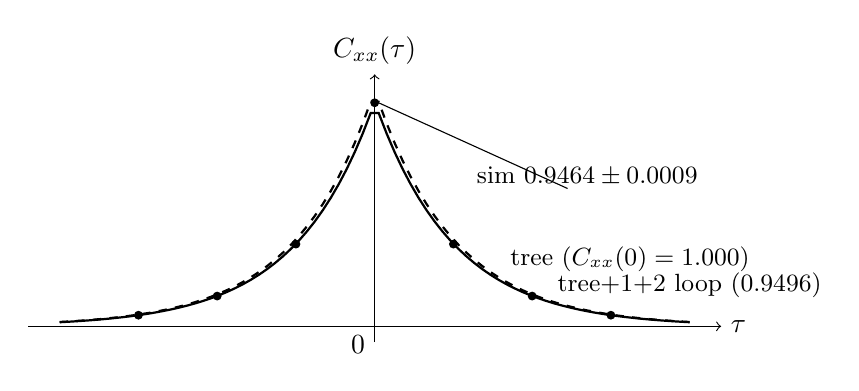
\begin{tikzpicture}[scale=1.0]
  % axes
  \draw[->] (-4.4,0) -- (4.4,0) node[right] {$\tau$};
  \draw[->] (0,-0.2) -- (0,3.2) node[above] {$C_{xx}(\tau)$};
  \node[below left] at (0,0) {$0$};
  % tree curve: 1.0 * exp(-|tau|), peak at 1.0 -> scaled to 3.0 box (1.0 == 3.0)
  \draw[thick, dashed]
    plot[domain=-4:4, samples=80] (\x, {3.0*exp(-abs(\x))});
  \node[right, font=\small] at (1.6,{3.0*exp(-1.6)+0.25}) {tree ($C_{xx}(0)=1.000$)};
  % loop-corrected curve: 0.9496 * exp(-|tau|)
  \draw[thick]
    plot[domain=-4:4, samples=80] (\x, {2.849*exp(-abs(\x))});
  \node[right, font=\small] at (2.2,{2.849*exp(-2.2)+0.2}) {tree+1+2 loop ($0.9496$)};
  % simulation points on the loop-corrected curve
  \foreach \x in {-3,-2,-1,0,1,2,3} {
    \fill (\x, {2.839*exp(-abs(\x))}) circle (1.6pt);
  }
  \node[font=\small] at (2.7,1.9) {sim $0.9464\pm0.0009$};
  \draw (2.45,1.75) -- (0.05,{2.839});
\end{tikzpicture}
\end{center}

(The real plot is a Matplotlib figure with proper axes and a legend; this sketch
just fixes the relationship between the three curves in your mind.)

\section{What you just did, and where to go next}

In six steps and a few dozen lines of code you:
\begin{enumerate}
  \item loaded a declarative theory file into a \code{(model, module)} pair;
  \item printed the model to confirm its fields, parameters, and saddle;
  \item packaged your choices --- $k=2$, two loops, the autocorrelator legs, the
        parameter values --- into a single \code{Config};
  \item drove the entire seven-phase \msrjd{} pipeline with one \code{run} call;
  \item read the loop-corrected equal-time variance ($0.9496$) off the result;
  \item validated it against an independent SDE simulation ($0.9464 \pm 0.0009$)
        and overlaid the two.
\end{enumerate}

Every step here was deliberately the easy case: a single temporal field, white
noise, a small loop parameter, a symmetric saddle at the origin. The rest of the
manual generalises each axis of that easy case. The chapters on the theory
specification and theory files explain how \code{build()},
\code{DEFAULT\_FUNDAMENTAL}, and \code{METADATA} are authored. The chapters on the
field-theory core, the propagator, the mean-field solve, diagram enumeration,
type assignment, and Phase~J open up the seven phases one at a time. The chapter
on cumulants and moments explains the \code{output='moment'} path we skipped. And
the spatial chapters take the same \code{load $\to$ Config $\to$ run $\to$ plot}
spine into PDEs, where the result is a $C(x,\tau)$ surface rather than a
$C(\tau)$ curve.

If you want to experiment right now, the most instructive single change is to push
$\mu$ toward $0$ (or below it, into the double well) in \code{Config.parameters}:
that grows the effective loop parameter $g_{\mathrm{eff}} = \varepsilon D/\mu^{2}$
and stresses the perturbative series, so you can watch tree, one-loop, and
two-loop pull apart on the plot --- and watch the agreement with the simulation
degrade as truncation starts to bite.
